\section{Реализация алгоритма Raft на TLA+}

TLA+ — язык спецификаций, основанный на теории множеств, логике первого порядка
и темпоральной логике действий (англ. TLA, temporal logic of actions).

Темпоральная логика была введена Амиром Пнуэли в 1970-х годах \cite{amir70}.
Лесли Лэмпорт увидел недостаточность этой идеи для описания систем целиком и
пришёл к мысли о необходимости использовать конечные автоматы, которым
придавался смысл формул темпоральной логики, описывающих все возможные
пути исполнения. Таким образом родилась идея темпоральной логики действий
(TLA), которая дополнила темпоральную логику следующим \cite{lamport08}:

\begin{itemize}
    \item инвариантность при повторении состояния;
    \item темпоральное использование кванторов существования;
    \item принятие в качестве атомарных формул не только предикатов состояния,
        но и формул действий.
\end{itemize}

TLA-спецификация — темпоральная формула, часто называемая $Spec$ и являющаяся
предикатом (утверждением) о поведении. Поведение представляет собой возможный
путь исполнения системы \cite{habrias06}.

Состоянием называется присваивание значений переменных, шагом называется пара
состояний. Теперь поведение можно представить как бесконечную последовательность
состояний, а шагами поведения можно назвать пару последовательных состояний
поведения. Предикатом состояния называется функция, результат которой —
логическое значение истина или ложь — соответствует утверждению о состоянии.
Действием называется функция, имеющая смысл предиката над шагом. В этой функции
участвуют как переменные первого шага, так и второго, которые обычно
отмечаются штрихом \cite{habrias06}.

$$
Spec \triangleq Init \wedge \Box [Next]_{(v_1, v_2, ..., v_n)}
$$

Здесь $Init$ — предикат состояния, $Next$ — действие, $v_i$ — переменные, $\Box$
— единственный в данной спецификации темпоральный оператор (истинно во всех
будущих состояниях).

TLC — это программа, которая по заданному TLA+ описанию системы и формулам
свойств перебирает состояния системы и определяет, удовлетворяет ли система
заданным свойствам.

Обычно работа с TLA+/TLC строится таким образом: описываем систему в TLA+,
формализуем в TLA+ интересные свойства, запускаем TLC для проверки. Таким
образом и будет строиться работа по описанию алгоритма консенсуса Raft.

\subsection{Формальная спецификация алгоритма}

Ниже приведён подробный разбор TLA+ спецификации алгоритма консенсуса Raft.
Текст разделён на логические блоки (константы, переменные, вспомогательные
функции, действия, спецификация и т.д.) в том порядке, в каком они
представлены в коде. Полный код спецификации приведен в Приложении А.

\subsubsection*{Константы}

На рис. \ref{fig:tla-01} описаны константы спецификации. Константы в TLA+
представляют собой неизменные в пределах спецификации значения . Они определяются
в начале спецификации TLA+ и не изменяют свои значения в ходе выполнения модели
системы. Константы используются для настройки параметров или значений
конфигурации, которые определяют поведение системы, но не изменяются при
изменении состояния системы. Они будут заданы в части "Проверка модели".

\begin{figure}
  \centering
  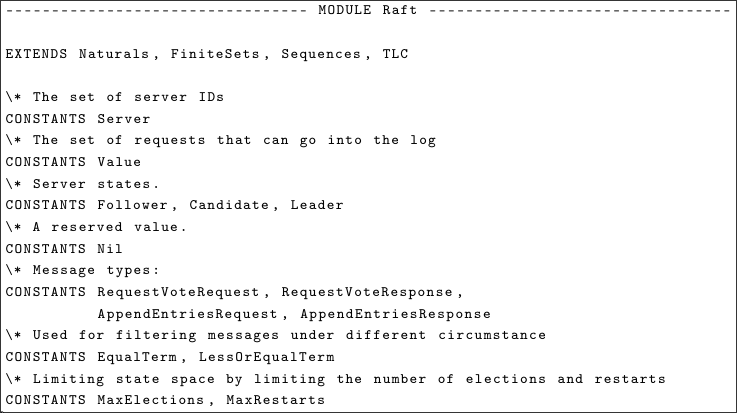
\includegraphics[scale=0.6]{inc/tla-01.png}
  \caption{Описание констант спецификации}
  \label{fig:tla-01}
\end{figure}

На рис. \ref{fig:tla-01} описана «основная среда» протокола: какие есть сервера,
значения, роли (Follower/Candidate/Leader), типы сообщений, специальные маркеры
вроде Nil и ограничения для упрощения моделирования.

$EXTENDS$ перечисляет, какие стандартные модули TLA+ были подключены:

\begin{itemize}
    \item $Naturals$: для работы с натуральными числами и базовыми операциями;
    \item $FiniteSets$: предоставляет операции над конечными множествами
        (например, $SUBSET(S)$);
    \item $Sequences$: даёт операции над последовательностями (например, $Len$,
        $Append$, $SubSeq$ и т.д.);
    \item $TLC$: вспомогательные средства моделирования (такие как $Permutations$,
        $Print$ и пр.), а также операторы типа $CHOOSE$.
\end{itemize}

$CONSTANTS$ $Server$ - множество идентификаторов серверов. Традиционно, когда
описывается система, состоящая из набора процессов/узлов, в TLA+ они задаются
как константа-множество (например, $\{s1, s2, s3\}$).

$CONSTANTS$ $Value$ – множество возможных «значений» (запросов), которые могут
добавляться в журналы (logs) серверов.

$\text{CONSTANTS Follower, Candidate, Leader}$ – три константы, обозначающие
состояния серверов в Raft: Последователь (Follower), Кандидат (Candidate)
и Лидер (Leader).

$CONSTANTS$ $Nil$ – специальное «пустое» значение. Применяется в случаях, когда
нужно указать «отсутствие чего-либо».

Блок ${CONSTANTS}$ $RequestVoteRequest$, $RequestVoteResponse$,
$AppendEntriesRequest$, $AppendEntriesResponse$ – четыре типа сообщений в Raft:
запрос на голосование, ответ на запрос голосования, запрос на добавления записей
в журнал и ответ на добавление соответственно.

$\text{CONSTANTS EqualTerm, LessOrEqualTerm}$ – два способа проверки периода (терма),
которые используются при обработке сообщений: равенство периодов (EqualTerm) или
меньшее/равное (LessOrEqualTerm).

$\text{CONSTANTS MaxElections, MaxRestarts}$ – ограничения для ограничения
пространства состояний (количество возможных выборов лидера и рестартов узлов).

\subsubsection*{Глобальные переменные}

Глобальная переменная (разделяемая между всеми серверами) только одна: $messages$.
Она представляет собой «мультимножество» сообщений, которые циркулируют в системе.
В коде это представлено как функция вида $Message \rightarrow Nat$, где $Nat$ –
сколько раз сообщение встречается (сколько копий есть в канале).

\subsubsection*{Вспомогательные переменные}

На рис. \ref{fig:tla-02} представлены вспомогательные переменные.

\begin{figure}
  \centering
  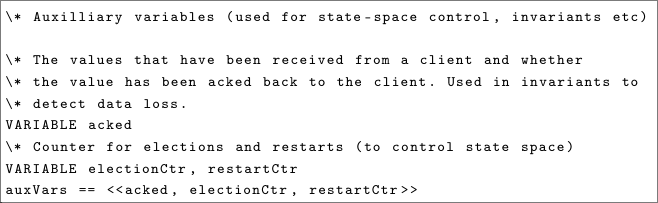
\includegraphics[scale=0.6]{inc/tla-02.png}
  \caption{Описание вспомогательных переменных}
  \label{fig:tla-02}
\end{figure}

$acked$ - это отображение вида $Value \rightarrow \{Nil, FALSE, TRUE\}$. Оно
показывает, было ли значение «подтверждено» (acked) сервером обратно клиенту.
Если $acked[v] = FALSE$, то запрос клиента уже поступил, но ещё не подтверждён;
если $TRUE$, то подтверждён. Если $Nil$, значит, это значение пока вообще не
предлагалось. Переменная используется в инвариантах для проверки отсутствия
потери данных.

$electionCtr$ и $restartCtr$ – счётчики, ограничивающие пространство состояний.
Определяют число выборов и рестартов, их максимальное значение задано константами
$MaxElections$, $MaxRestarts$, которые были описаны выше.

\subsubsection*{Переменные сервера}

Все переменные, приведенные на рис. \ref{fig:tla-03} определены для каждого
сервера. Т.е. каждая из них - функция от идентификатора сервера, задаваемого
констатами в $Server$.

\begin{figure}
  \centering
  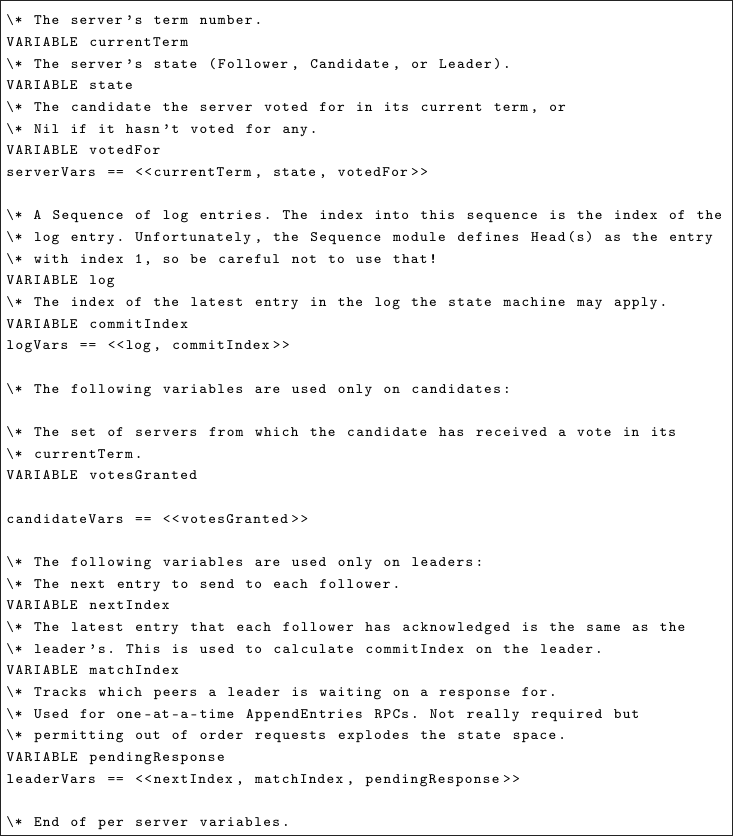
\includegraphics[scale=0.6]{inc/tla-03.png}
  \caption{Переменные сервера}
  \label{fig:tla-03}
\end{figure}

$currentTerm$ – для каждого сервера i хранит номер (терм) текущего периода Raft.
$state$ – текущее состояние сервера: $Follower$, $Candidate$ или $Leader$, как
было указано в константах.

$votedFor$ - для каждого сервера хранит, кому он отдал голос в текущем терме
(или Nil, если ещё не голосовал). Все они сгруппированы в переменную $serverVars$
для удобства обращения (например, в $WF\_vars(Next)$).

$log$ - функция от $Server$, где каждому серверу ставится в соответствие
последовательность ($Sequence$) записей в журнале. Элемент журнала обычно
содержит $(term, value)$.

$commitIndex$ показывает, до какого индекса журнал считается подтвержденнным
(т.е. готовым к применению к машине состояний).

$votesGranted$ – для сервера, который находится в состоянии $Candidate$, здесь
хранится множество серверов, которые этому кандидату дали голос в текущем терме.

$nextIndex$ – для каждого лидера и для каждого сервера в кластере хранит индекс,
с которого лидер должен отправлять записи в лог для репликации. То есть,
если $nextIndex[i][j] = k$, значит лидер $i$ собирается отправить серверу $j$ записи,
начиная с индекса $k$ (в логе самого лидера).

$matchIndex$ – для лидера $i$ и сервера $j$ указывает, до какого индекса журнала
сервер $j$ гарантированно имеет те же записи, что и лидер.

$pendingResponse$ – для лидера $i$ и сервера $j$ это булево значение, показывающее,
ждет ли лидер ответа на предыдущий RPC. Если $TRUE$, значит лидер уже отправил запрос
$AppendEntries$ серверу $j$ и ещё не получил ответа; чтобы в модели не плодилось
слишком много состояний, запрещено отправлять параллельные $AppendEntries$ одному
и тому же серверу.

\subsubsection*{Вспомогательные функции}

Реализация всех вспомогательных функций представлена на рис. \ref{fig:tla-04}.
Они не используются в инициализации системы, пересылке или обработке сообщений.

$Quorum$ – множество всех подмножеств серверов, которые образуют мажоритарный
кворум (подмножество, размер которого более половины). Если размер кластера $N$,
то в кворуме строго более $N/2$ узлов. Каждый кворум пересекается с любым другим
кворумом хотя бы в одном узле.

$LastTerm(xlog)$ – возвращает терм последней записи в журнале, или 0, если журнал
пуст.

$\_SendNoRestriction(m)$ – отправить сообщение $m$, увеличив счётчик копий в
$messages$. Если сообщение уже есть, увеличим счётчик, если нет – добавим новую
запись $m :> 1$.

\begin{figure}
  \centering
  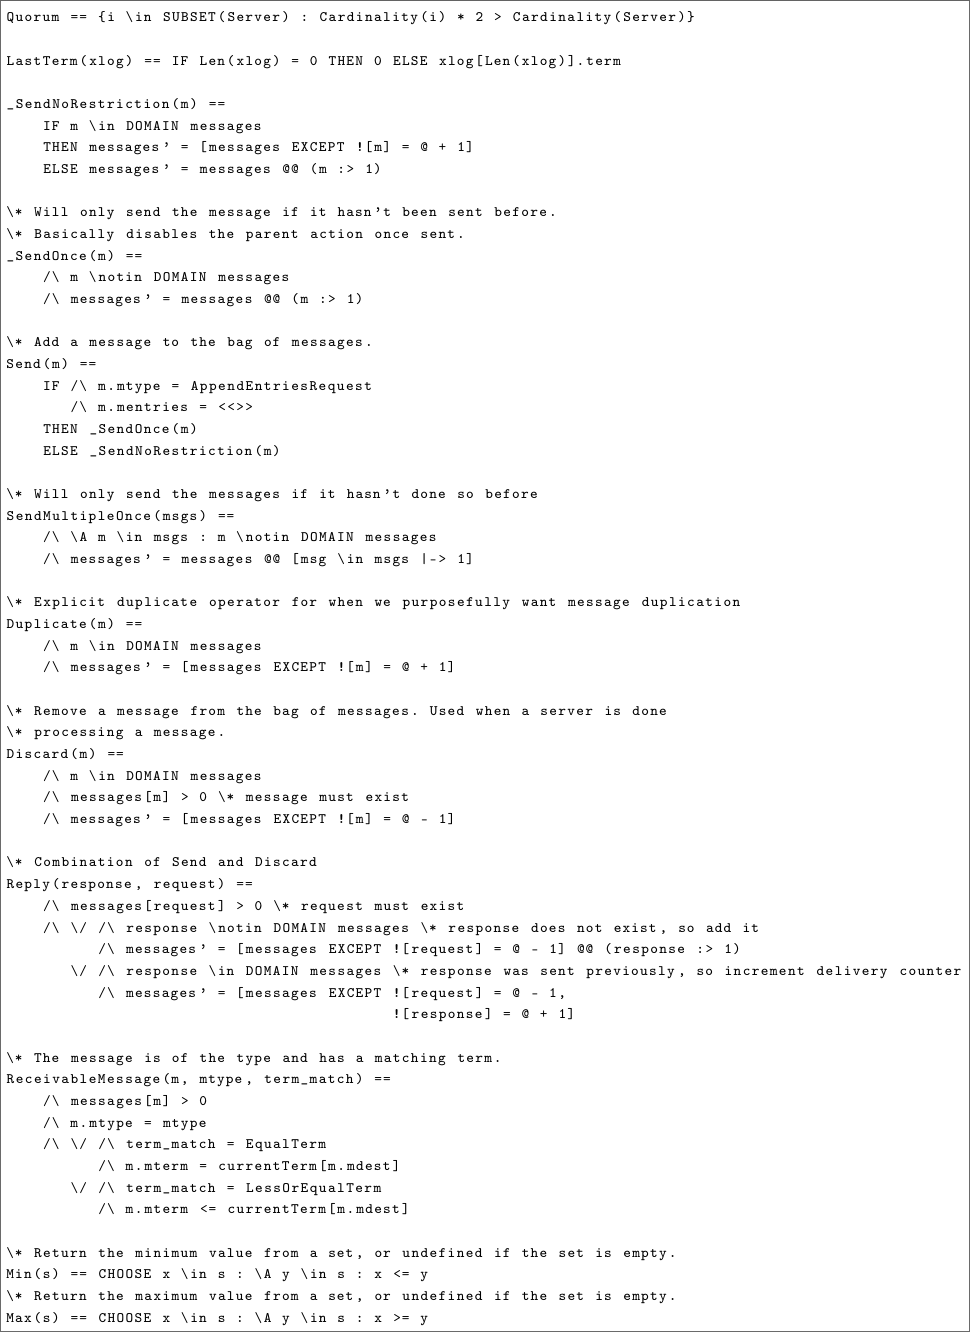
\includegraphics[scale=0.5]{inc/tla-04.png}
  \caption{Вспомогательные функции}
  \label{fig:tla-04}
\end{figure}

$\_SendOnce(m)$ – отправить сообщение m только один раз. Действие разрешено
только если такого сообщения ещё нет в $messages$. Это используется для тех
случаев, когда повторная отправка может сильно увеличивать пространство состояний
(например, пустые RPC не должны слаться бесконечно).

$Send(m)$ – оператор отправки сообщения. Если это $AppendEntriesRequest$ без
данных ($mentries=<<>>$), то используем правило «послать только один раз»; иначе
же можно добавлять в мешок сколько угодно раз.

$SendMultipleOnce(msgs)$ – отправляем сразу несколько сообщений за один шаг, но
только если ни одно из них ранее не присутствовало. Множество $msgs$ – набор
сообщений (часто это рассылка $RequestVote$ всем остальным).

$Duplicate(m)$ – искусственно дублирует сообщение, увеличивая его счётчик.
Это отдельное действие «сеть может продублировать сообщение».

$Discard(m)$ – «убрать одно вхождение сообщения из мешка». Если там несколько
копий, счётчик уменьшится на 1. Обычно вызывается после обработки сообщения
сервером.

$Reply(response, request)$ – соединяет операцию «удалить входящее сообщение
$(request)$» и «положить/увеличить ответ (response)» за один шаг. Если ответ уже
существует, увеличиваем счётчик; если нет – добавляем.

$Min/Max$ – функции для выборки минимального/максимального элемента из множества.

\subsubsection*{Инициализация}

На рис. \ref{fig:tla-05} представлена инициализация модели, по выполнении которой
формируется полное начальное состояние Raft-кластера: все сервера Follower’ы с
термом 1, без записей в журнале, без активных сообщений и с нулевыми счётчиками.

Важно отметить, что все переменные, кроме $electionCtr$, $restartCtr$, $acked$ и
$messages$ объявляются как функция от $Server$ ($\text{i in Server |->}$), можно
воспринимать их также как таблицу $map$.

\begin{figure}
  \centering
  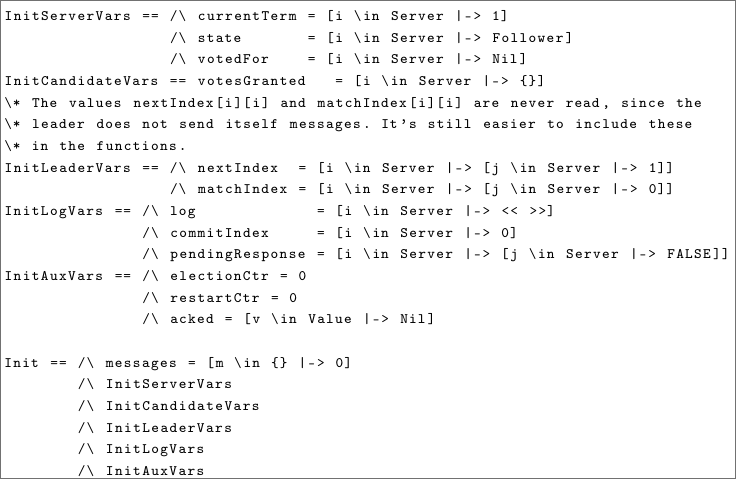
\includegraphics[scale=0.6]{inc/tla-05.png}
  \caption{Инициализация модели}
  \label{fig:tla-05}
\end{figure}

\subsubsection*{Действия}

В Raft есть несколько ключевых переходов. Каждый переход описывает, при каких
условиях он выполняется и как меняет состояние. Затем все они объединяются в
оператор $Next$, который говорит: «возможен любой из этих переходов».

\textbf{Restart}

Код метода $Restart$ представлен на рис. \ref{fig:tla-06-restart}. Он переводит
сервер в состояние $Follower$, сбрасывает все «volatile» переменные ($votesGranted$,
$nextIndex$, $matchIndex$, $pendingResponse$, $commitIndex$), увеличивает счётчик
$restartCtr$. При этом не изменяются «persistent» переменные: терм ($currentTerm[i]$),
$votedFor[i]$, сам журнал ($log[i]$), уже подтверждённые значения. Условие
$restartCtr < MaxRestarts$ ограничивает количество рестартов.

\begin{figure}
  \centering
  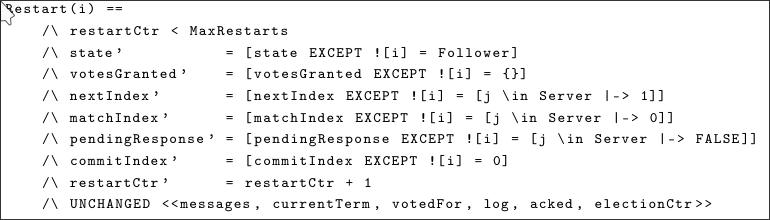
\includegraphics[scale=0.4]{inc/tla-06-restart.png}
  \caption{Метод $Restart$}
  \label{fig:tla-06-restart}
\end{figure}

\textbf{RequestVote}

Код метода $RequestVote$ представлен на рис. \ref{fig:tla-06-request-vote}. Сервер
$i$ будучи в состоянии $Follower$ или $Candidate$, начинает новые выборы следующим
образом:

\begin{enumerate}
    \item Проверка, что ещё не превышен $MaxElections$;
    \item Состояние меняется в $Candidate$;
    \item Терм увеличивается на 1;
    \item Отдается голос самому себе: $votedFor[i] = i$;
    \item Увеличивается счетчик выборов;
    \item Рассылаются запросы на голос всем серверам, кроме себя ($RequestVoteRequest$).
\end{enumerate}

\begin{figure}
  \centering
  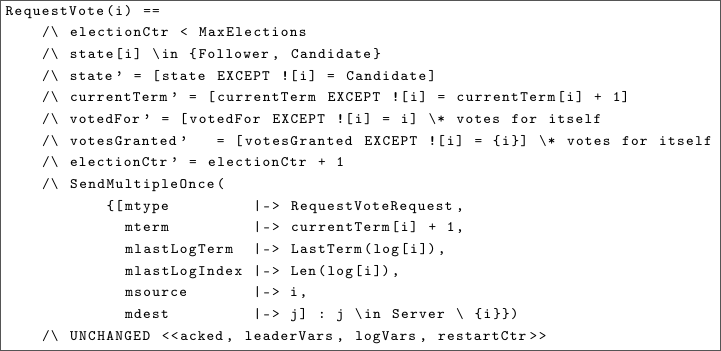
\includegraphics[scale=0.4]{inc/tla-06-request-vote.png}
  \caption{Метод $RequestVote$}
  \label{fig:tla-06-request-vote}
\end{figure}

\textbf{AppendEntries}

Код метода $AppendEntries$ представлен на рис. \ref{fig:tla-06-append-entries}.

\begin{figure}
  \centering
  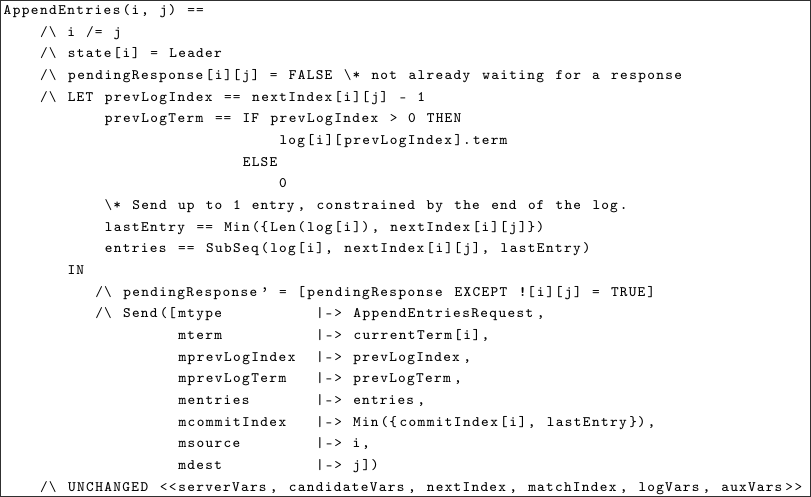
\includegraphics[scale=0.4]{inc/tla-06-append-entries.png}
  \caption{Метод $AppendEntries$}
  \label{fig:tla-06-append-entries}
\end{figure}

Лидер $i$ отправляет запрос $AppendEntriesRequest$ последователю $j$. В сообщении
не может быть больше одной записи $entry$. Условие $\text{pendingResponse[i][j] = FALSE}$
гарантирует, что не отправляем новый RPC, пока старый еще без ответа.

\textbf{BecomeLeader}

Код метода $BecomeLeader$ представлен на рис. \ref{fig:tla-06-become-leader}.
Сервер-кандидат $i$ обнаруживает, что у него есть кворум голосов (в $votesGranted[i]$).
Значит, он выигрывает выборы и становится лидером. Переводится $state[i]$ в $Leader$,
инициализируется $nextIndex[i]$, $matchIndex[i]$, $pendingResponse[i]$. Другие
переменные не меняются.

\begin{figure}
  \centering
  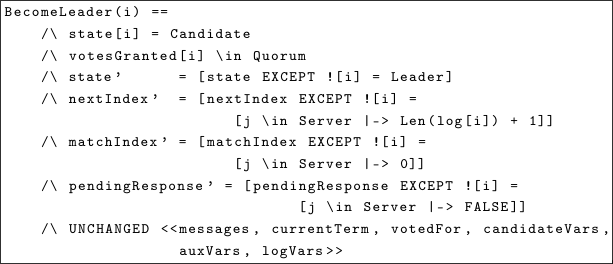
\includegraphics[scale=0.4]{inc/tla-06-become-leader.png}
  \caption{Метод $BecomeLeader$}
  \label{fig:tla-06-become-leader}
\end{figure}

\textbf{AdvanceCommitIndex}

Код метода $AdvanceCommitIndex$ представлен на рис. \ref{fig:tla-06-advance-commit-index}.

\begin{figure}
  \centering
  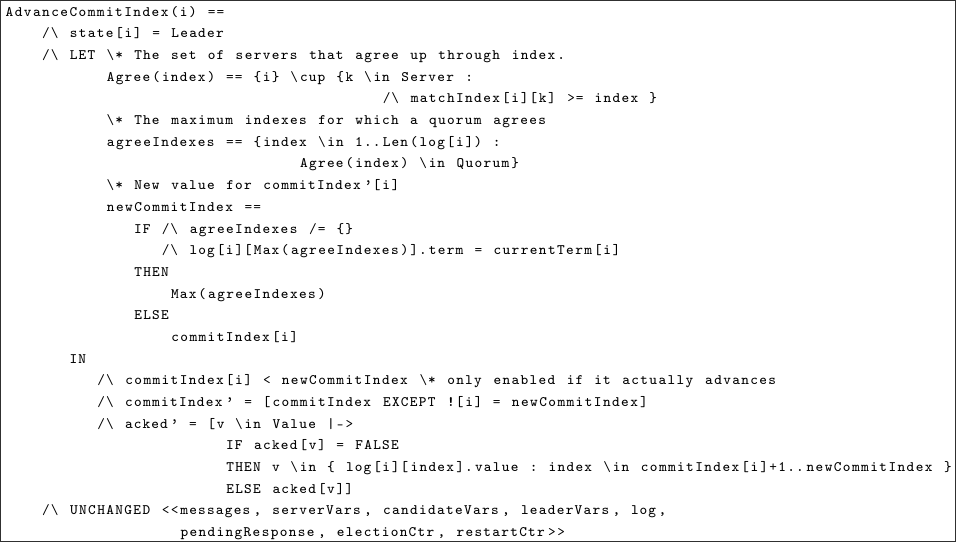
\includegraphics[scale=0.4]{inc/tla-06-advance-commit-index.png}
  \caption{Метод $AdvanceCommitIndex$}
  \label{fig:tla-06-advance-commit-index}
\end{figure}

Лидер $i$ пытается продвинуть свой $commitIndex$ вперёд, если есть подтверждение
большинства узлов для определённого индекса. Для этого проверяется множество
серверов, у которых $matchIndex[i][k] >= index$, и вычисляется максимум индексов,
по которым у лидера есть кворум. Если этот индекс принадлежит текущему терму лидера,
обновляется $commitIndex[i]$. Все значения, которые таким образом становятся
закоммиченными, теперь помечаются $acked[v] = TRUE$.

\textbf{UpdateTerm}

Код метода $UpdateTerm$ представлен на рис. \ref{fig:tla-06-update-term}.
Если где-то в сети есть сообщение с термом больше, чем у сервера, который
его получит, то сервер «обновляет» свой терм, сбрасывает своё голосование,
становится $Follower$.

\begin{figure}
  \centering
  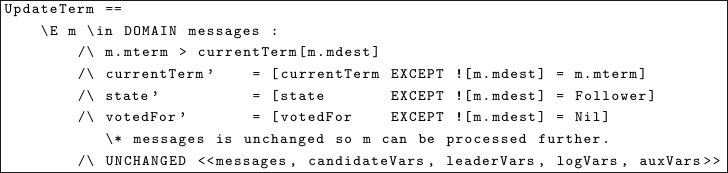
\includegraphics[scale=0.4]{inc/tla-06-update-term.png}
  \caption{Метод $UpdateTerm$}
  \label{fig:tla-06-update-term}
\end{figure}

\textbf{HandleRequestVoteRequest}

Код метода $HandleRequestVoteRequest$ представлен на рис. \ref{fig:tla-06-handle-request-vote}.

\begin{figure}
  \centering
  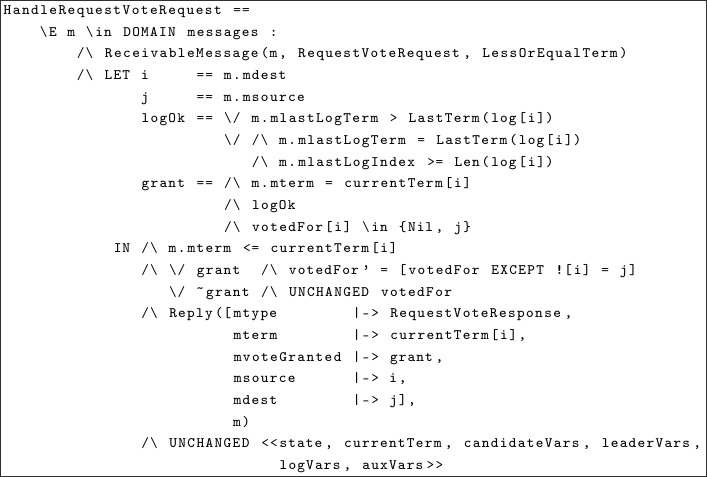
\includegraphics[scale=0.4]{inc/tla-06-handle-request-vote.png}
  \caption{Метод $HandleRequestVoteRequest$}
  \label{fig:tla-06-handle-request-vote}
\end{figure}

Сервер $i$ обрабатывает входящий $RequestVoteRequest$ от сервера $j$. Сначала
проверяется условие $\textit{ReceivableMessage(..., LessOrEqualTerm)}$, то есть
терм запроса не больше текущего, иначе этим занялось бы $UpdateTerm$. Затем
проверяется «лог последнего кандидата»: \textit{(m.mlastLogTerm, m.mlastLogIndex)}
сравнивается с собственным журналом. Если лог кандидата не меньше нашего, и сам
сервер $i$ ещё не голосовал в этом терме (или уже голосовал за $j$), мы отдадим
ему голос. Результат — отправка $RequestVoteResponse$ с $mvoteGranted = grant$.

\textbf{HandleRequestVoteResponse}

Код метода $HandleRequestVoteResponse$ представлен на рис.
\ref{fig:tla-06-handle-request-vote-response}. Сервер $i$ получает ответ на
запрос голосования от $j$. Если $mvoteGranted = TRUE$, добавляем $j$ в
$votesGranted[i]$. Иначе ничего не делаем. Сообщение удаляется из сети после
обработки.

\begin{figure}
  \centering
  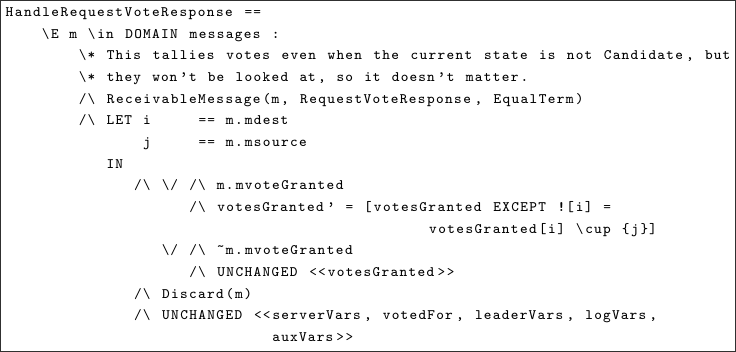
\includegraphics[scale=0.4]{inc/tla-06-handle-request-vote-response.png}
  \caption{Метод $HandleRequestVoteResponse$}
  \label{fig:tla-06-handle-request-vote-response}
\end{figure}

\textbf{RejectAppendEntriesRequest}

Код метода $RejectAppendEntriesRequest$ представлен на рис.
\ref{fig:tla-06-reject-append-entries}.
Сервер $i$ отвергает $AppendEntriesRequest$, если терм сообщения меньше его
собственного либо если термы равны, но у получателя – $Follower$, и при этом
журнал «не совпадает» (поле $m.mprevLogTerm$ или $m.mprevLogIndex$ не
соответствуют локальному журналу).

\begin{figure}
  \centering
  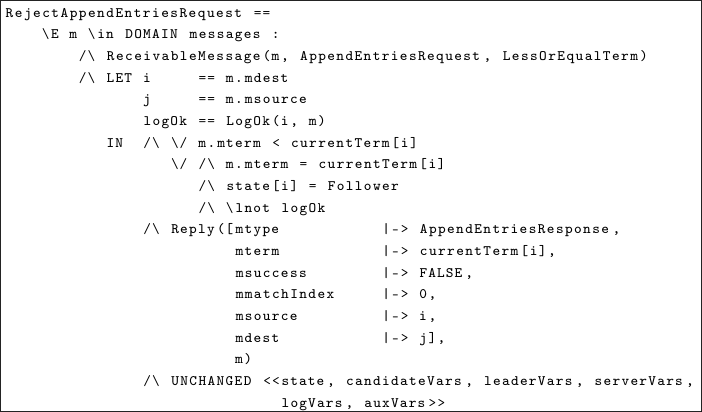
\includegraphics[scale=0.4]{inc/tla-06-reject-append-entries.png}
  \caption{Метод $RejectAppendEntriesRequest$}
  \label{fig:tla-06-reject-append-entries}
\end{figure}

В ответ отправляется $AppendEntriesResponse$ с $msuccess = FALSE$.

\textbf{AcceptAppendEntriesRequest}

Код метода $AcceptAppendEntriesRequest$ представлен на рис.
\ref{fig:tla-06-accept-append-entries}.
Может произойти урезание лога и/или добавление одной записи. $commitIndex'[i]$
устанавливается равным тому, что лидер прислал в $m.mcommitIndex$, так как
$Follower$ следует за лидером. Отправляем положительный ответ ($AppendEntriesResponse$)
с $msuccess = TRUE$.

\begin{figure}
  \centering
  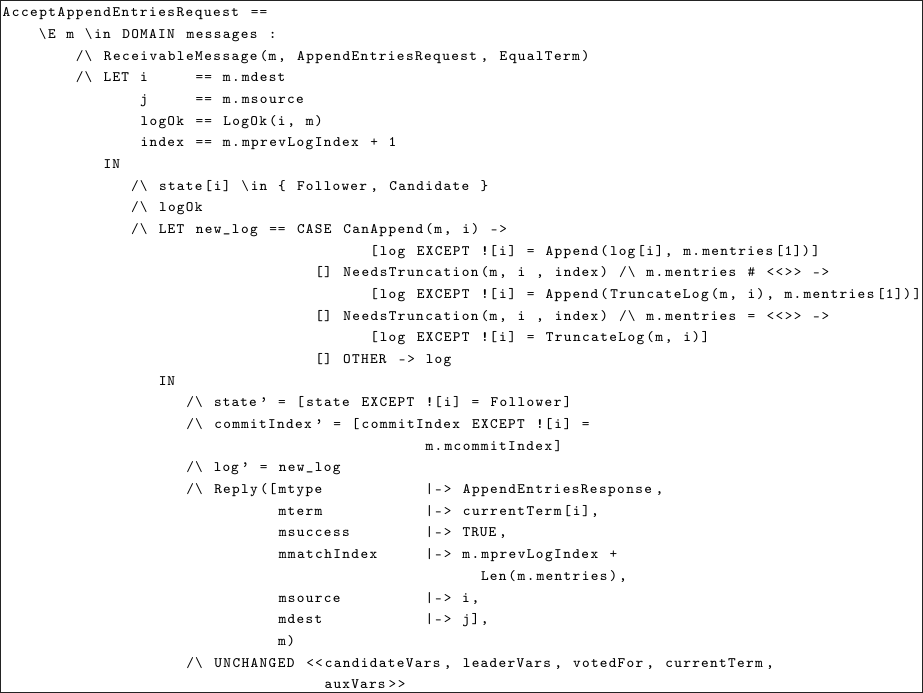
\includegraphics[scale=0.4]{inc/tla-06-accept-append-entries.png}
  \caption{Метод $AcceptAppendEntriesRequest$}
  \label{fig:tla-06-accept-append-entries}
\end{figure}

\textbf{HandleAppendEntriesResponse}

Код метода $HandleAppendEntriesResponse$ представлен на рис.
\ref{fig:tla-06-handle-accept-append-entries-response}.

\begin{figure}
  \centering
  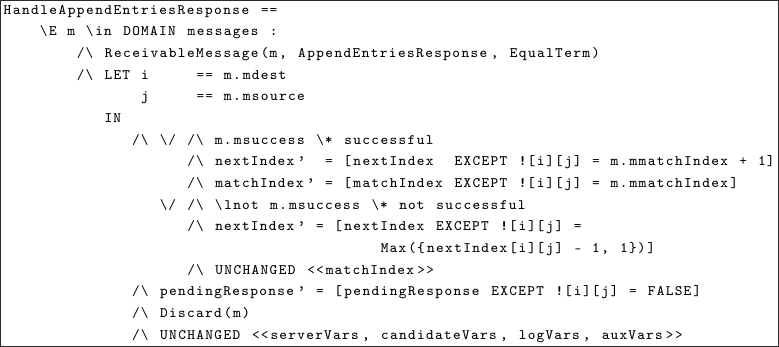
\includegraphics[scale=0.4]{inc/tla-06-handle-append-entries-response.png}
  \caption{Метод $HandleAppendEntriesResponse$}
  \label{fig:tla-06-handle-append-entries-response}
\end{figure}

Лидер $i$ получает ответ от $j$. Если $m.msuccess = TRUE$, значит $j$ у себя
добавил записи, и лидер ставит $matchIndex[i][j] = mmatchIndex$. $nextIndex[i][j]$
становится $mmatchIndex + 1$. Если $FALSE$, значит у $j$ оказались расхождения,
и тогда лидер уменьшает $nextIndex[i][j]$ на 1, чтобы попробовать снова.
$pendingResponse'[i][j] = FALSE$ – освобождается «окно» для следующего запроса.
Затем сообщение выбрасывается из сети.

\subsubsection*{Спецификация и оператор Next}

Код оператора и спецификации приведен на рис. \ref{fig:tla-07}

\begin{figure}
  \centering
  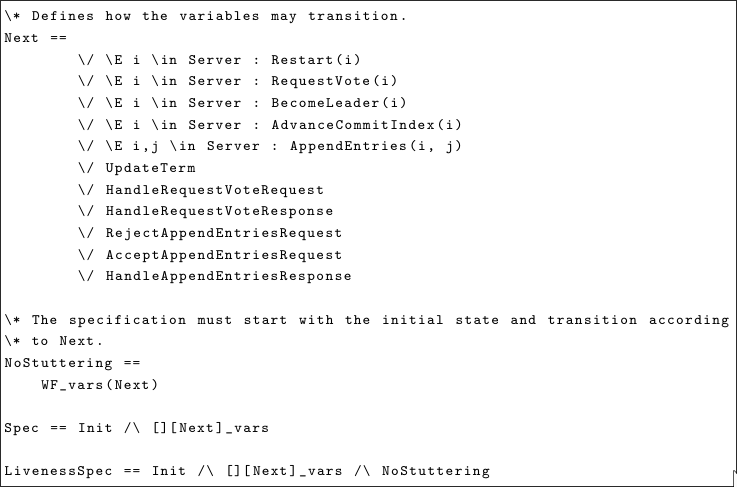
\includegraphics[scale=0.4]{inc/tla-07.png}
  \caption{Спецификация и оператор $Next$}
  \label{fig:tla-07}
\end{figure}

Оператор $Next$ представляет собой главную дизъюнкцию всех возможных действий,
которые могут происходить в любой момент. Система в каждый момент времени может
сделать один из перечисленных переходов (\textit{Restart, RequestVote, AppendEntries,
BecomeLeader} и т.п.), если выполняются условия.

$Spec$ – классическая структура TLA+ спецификации: $Init$ задаёт начальное
состояние, $[][Next]\_vars$ говорит, что на каждом шаге выполняется одно из
действий $Next$.

\subsubsection*{Инварианты}

Инварианты представлены на рис. \ref{fig:tla-08}. Они проверяются моделью, описанной
в следующей части, чтобы убедиться, что Raft-свойства не нарушаются при любых
последовательностях действий.

\begin{figure}
  \centering
  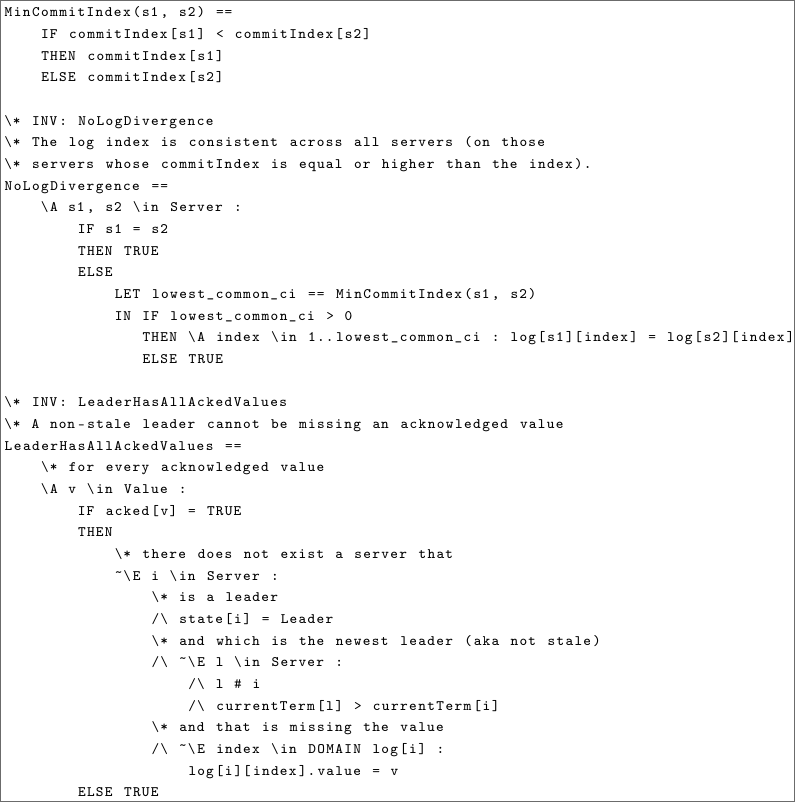
\includegraphics[scale=0.4]{inc/tla-08.png}
  \caption{Инварианты}
  \label{fig:tla-08}
\end{figure}

$NoLogDivergence$ – инвариант о том, что если у двух серверов некий индекс
подтвержден (меньшее из их commitIndex), то записи по этому индексу совпадают.
Это ключевое свойство согласованности в Raft.

$LeaderHasAllAckedValues$ – если значение ($v$) уже подтверждено как
$acked[v] = TRUE$, то любой лидер обязан иметь это значение в своём логе.

\subsubsection*{Итого}

Данная спецификация описывает основные аспекты Raft:

\begin{enumerate}
    \item Состояния узлов (\textit{Follower, Candidate, Leader}) и их персистентные
        переменные (\textit{currentTerm, votedFor, log}).
    \item Обмен сообщениями (\textit{RequestVote, AppendEntries} и их ответы) через
        переменную $messages$.
    \item Логика перехода (кандидат пытается стать лидером, лидер реплицирует
        записи, узлы отвечают и обновляют термы, если видят более высокий терм,
        и т.д.).
    \item Инварианты (\textit{NoLogDivergence, LeaderHasAllAckedValues}, и пр.),
        которые отражают ключевые свойства безопасности Raft.
\end{enumerate}

Таким образом, в модели учтены основные механизмы Raft: выбор лидера, поддержка
согласованного журнала, коммиты и гарантии о том, что система не теряет
записанные и закоммиченные данные.

\subsection{Проверка модели}

В TLA+ модель проверяется с помощью TLC, перебирающего всевозможные (или
ограниченные) пути выполнения спецификации и проверяющего инварианты.

В приложении Б приведен код конфигурации модели для TLC, в котором задаются
значения констант, какие варианты проврять, какой оператор считать стартовым и
переходным.

Результаты проверки приведены на рис. \ref{fig:tla-09}. Было проверено более 36
тысяч возможных состояний, инварианты не нарушаются.

\begin{figure}
  \centering
  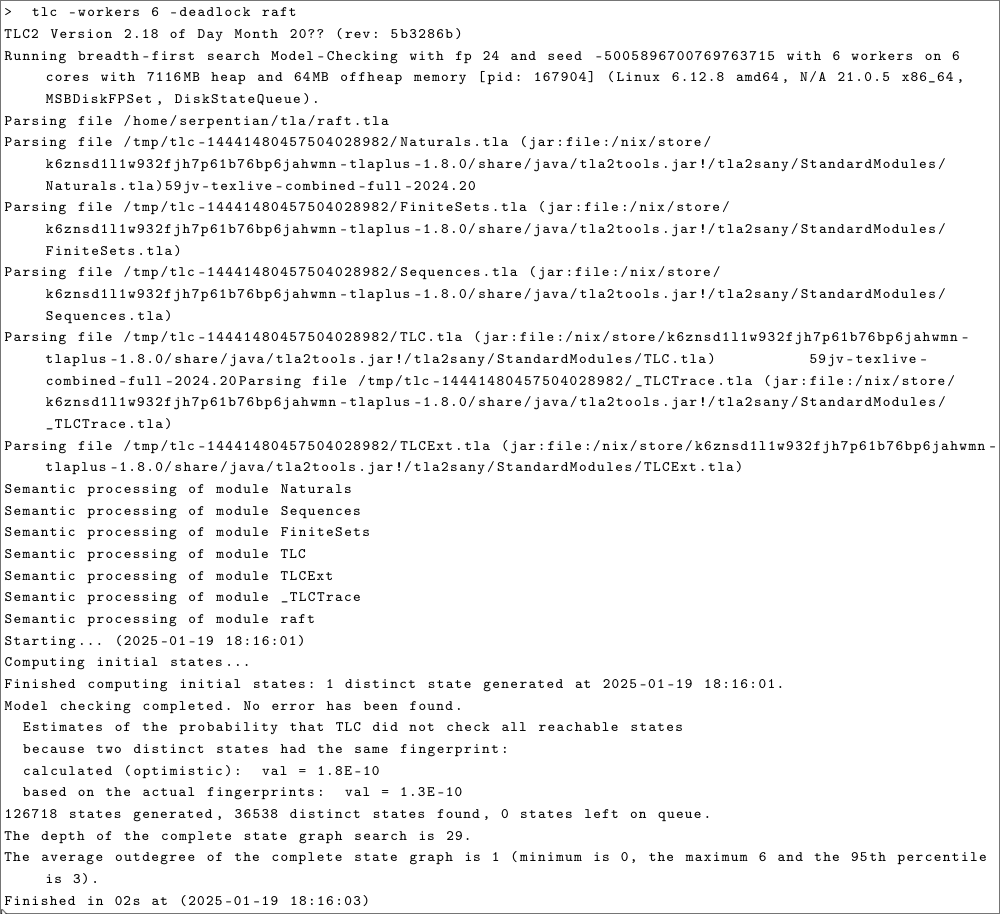
\includegraphics[scale=0.4]{inc/tla-09.png}
  \caption{Проверка модели}
  \label{fig:tla-09}
\end{figure}
